\documentclass[final]{beamer}
\mode<presentation>
{
  \usetheme{Szeged}
\usecolortheme{crane}
}


\usepackage{times}
\usepackage{multicol}
\usepackage{amsmath,amssymb,amsthm}

\newtheorem{alg}{Algorithm}

\newcommand{\argmax}{\text{argmax}}
\usepackage{float, caption, subcaption}
\usepackage[english]{babel}
\usepackage[latin1]{inputenc}
\usepackage{beamerposter}  % e.g. custom size poster
  \title[]{{\veryHuge An Optimization Layer for Distributed Matrix Computations }}
  \author[]{{\Large Jonah Brown Cohen, Tselil Schramm, and Ben Weitz}}
\date{}

  \begin{document}
{\large
  \begin{frame}{} 

\maketitle

\vspace{-1cm}
\begin{center}
\begin{columns}[t]
\begin{column}{0.32\textwidth}

%----------------------------------------------------------------------------------

    \begin{block}{\huge Motivation}
\vspace{.5cm}
{\Large Companies like Facebook, Netflix, and Google perform large-scale distributed matrix computations}
\begin{columns}[t]
\begin{column}{0.45\textwidth}
\begin{itemize} {\Large
\item Trade-offs: accuracy vs. time vs. money
\item Humans: bad at choosing parameters
\item Solution: an optimization layer to automatically manage computations
\item Learn from past computations
\item Meet time, accuracy, or monetary budget
}
\end{itemize}
\end{column}
\begin{column}{0.45\textwidth}
\begin{center}
\begin{figure}
\fbox{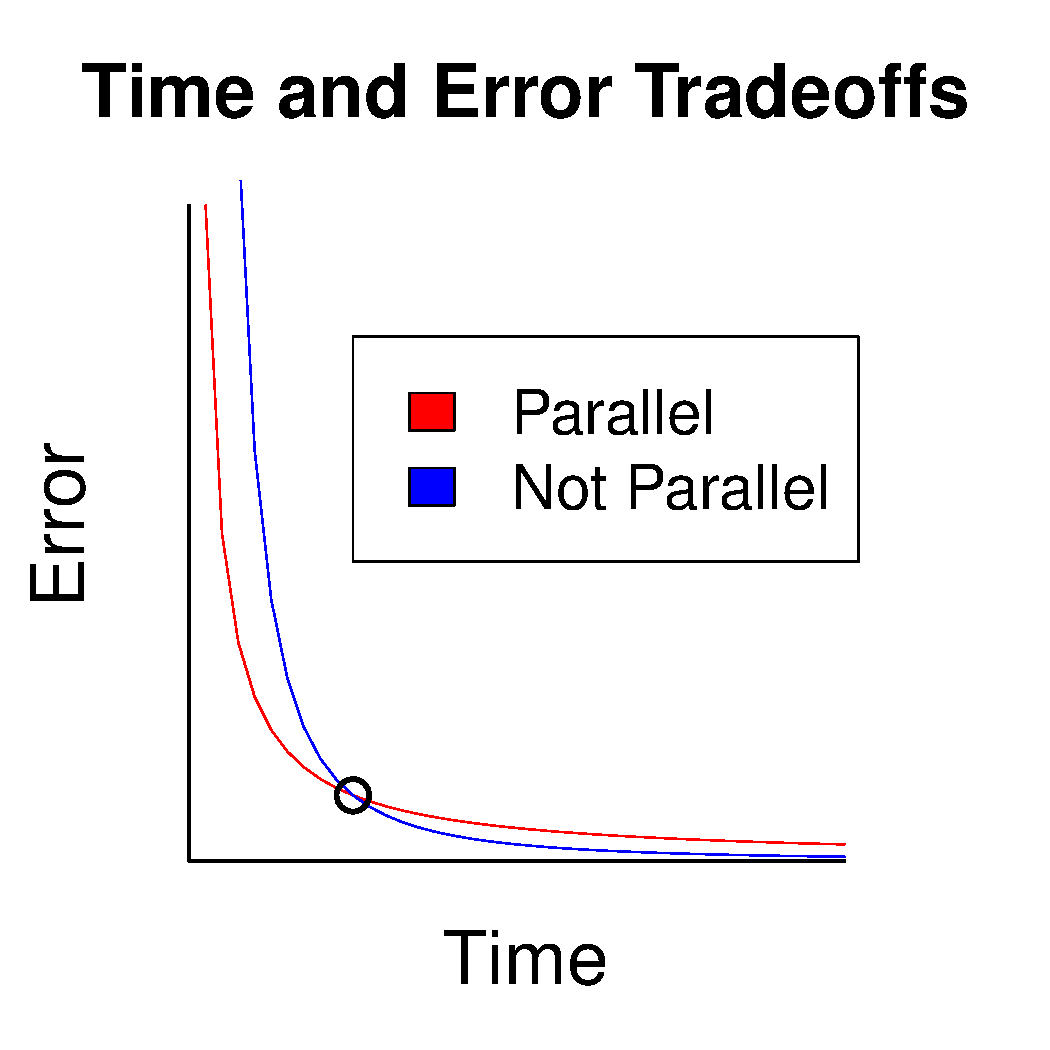
\includegraphics[width=0.9\textwidth]
{Motivations.pdf}}
\caption{Tradeoffs between time and error as more parallelism is used.}
\end{figure}
\end{center}
\end{column}
\end{columns}
\vspace{1.0cm}

\end{block}
\vspace{1.8cm}

    \begin{block}{\huge Objective}
\vspace{.6cm}
	{\bf \Large Automate the choice of algorithm parameters and number of partitions to meet time, accuracy, and monetary budget specifications}

\vspace{.6cm}

\end{block}

\vspace{1.8cm}

    \begin{block}{\huge Framework}
\vspace{.5cm}
\begin{columns}[t]
\begin{column}{0.45\textwidth}
	\vspace{2cm}
\begin{itemize}{\Large
\item User specifies input data, and time, error, and monetary budgets
\item Optimizer then interfaces with algorithms implemented on top of a parallel framework
\item All parameter selection hidden from user
}
\end{itemize}    
\end{column}
\begin{column}{.5\textwidth}
\begin{center}
\begin{figure}
\fbox{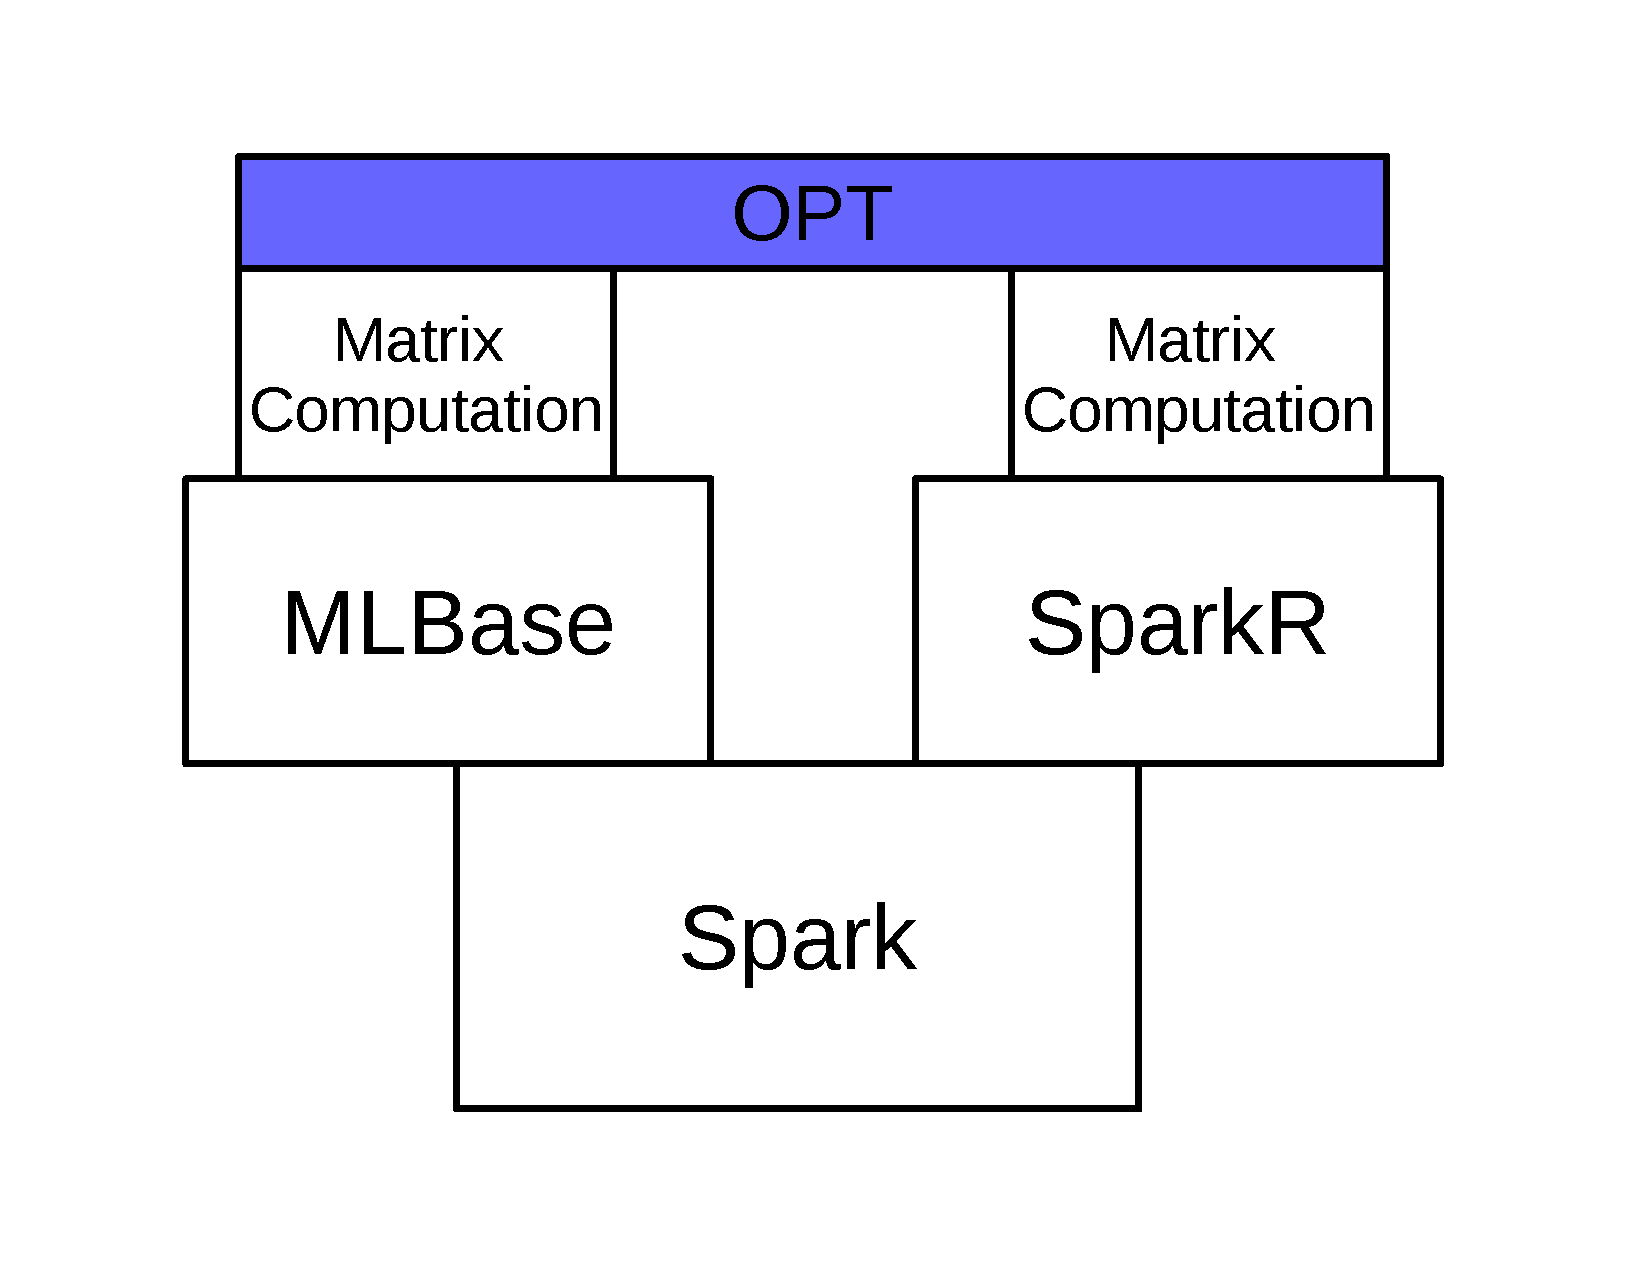
\includegraphics[width=0.9\textwidth]
{SysDiagram.pdf}}
\caption[width=\textwidth]{The information and control flow of distributed matrix computations with the aid of the optimizer.}
\end{figure}
\end{center}
\end{column}
\end{columns}
\end{block}

%----------------------------------------------------------------------------------

\vspace{1.2cm}

   
\end{column}

\begin{column}{0.32\textwidth}
 
    \begin{block}{\huge Optimizer Design}
\vspace{.5cm}

{\Large Optimizer stores statistics from prior jobs}
\begin{itemize}{\Large
\item Architecture-independent
\begin{itemize} {\Large
\item Parameters chosen based on statistics from prior jobs on the same architecture
}
\end{itemize}
\vspace{.5cm}

\item Adaptive
\begin{itemize} {\Large
\item Predictions for data from a specific distribution improve as the optimizer learns
}
\end{itemize}
\vspace{.5cm}

\item Avoids Local Optima
\begin{itemize} {\Large
\item When there is variation in results, there is a risk of getting stuck at a local optimum
\item In ``explore mode'' we add randomness: parameters are chosen with probability proportional to their relative suitability
}
	\end{itemize}}
\end{itemize}

\vspace{.7cm}

\begin{center}
\begin{figure}
\fbox{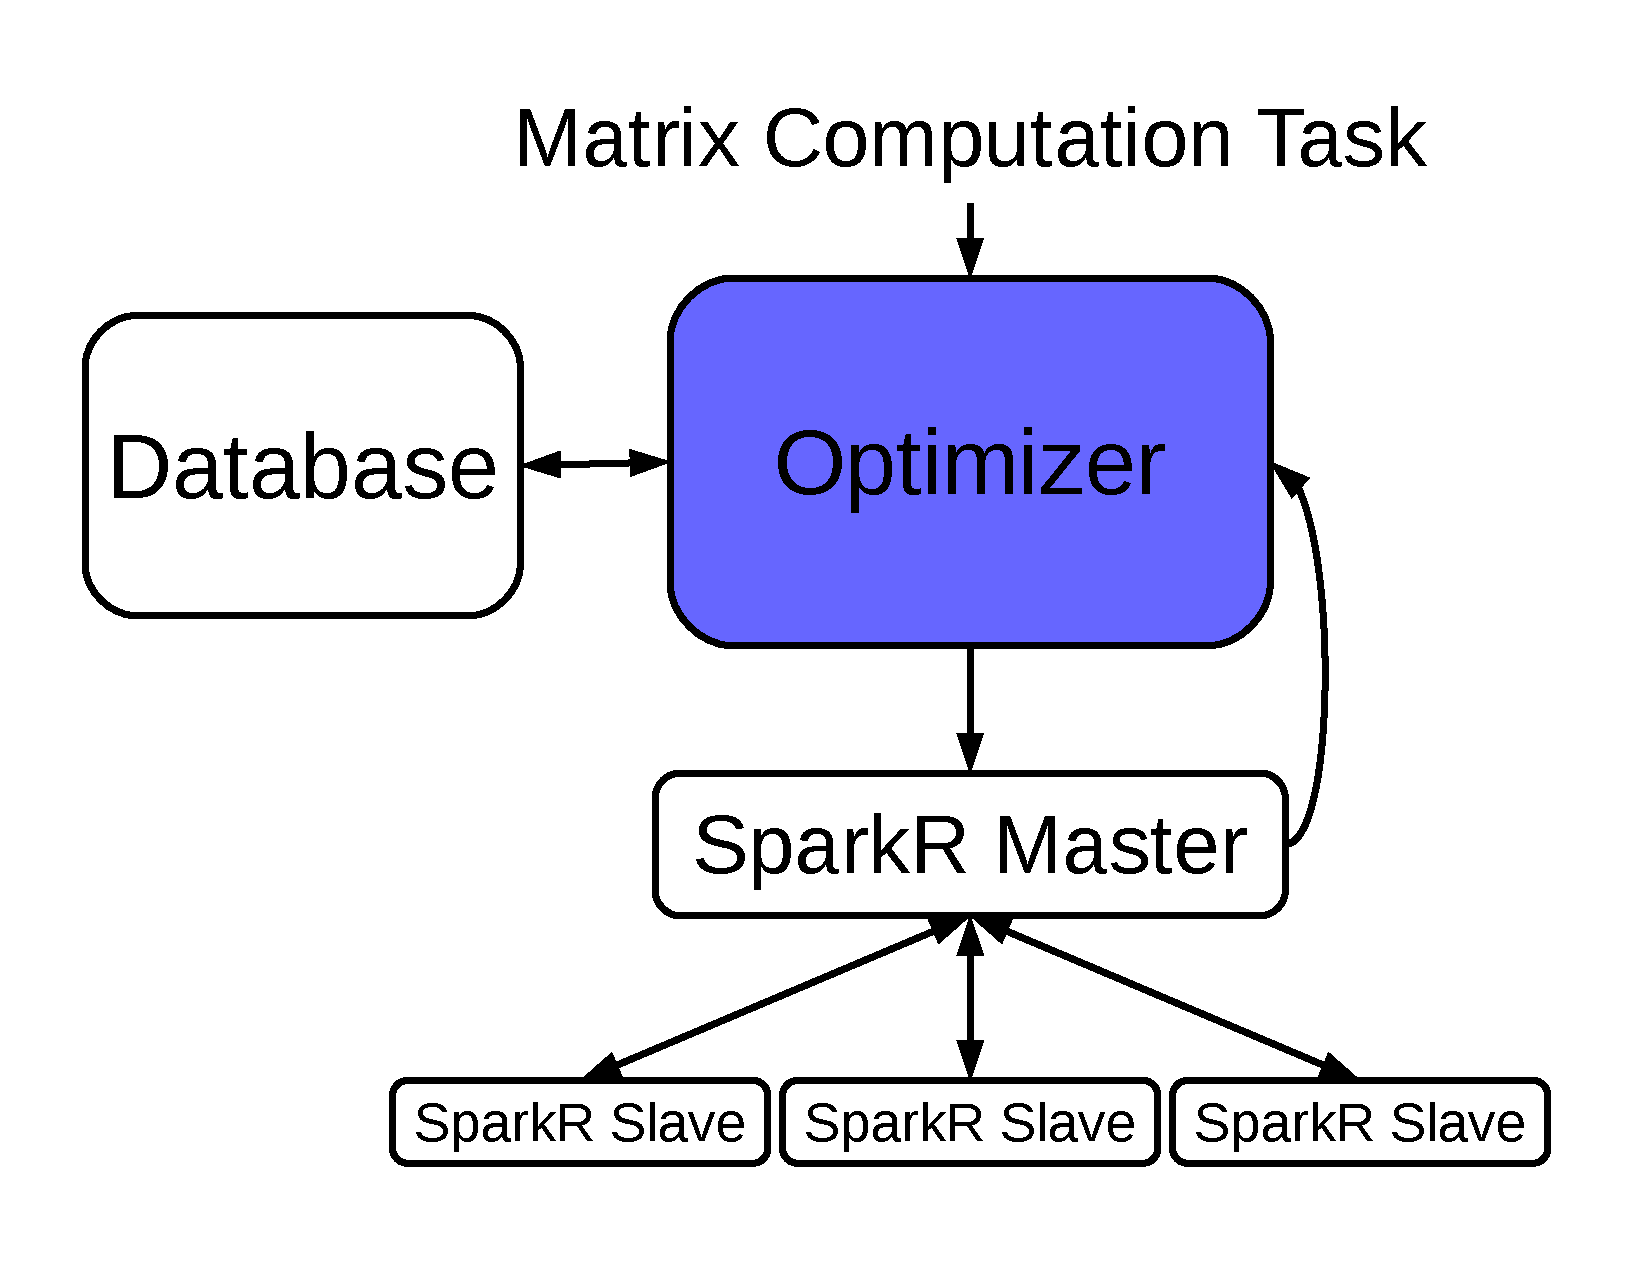
\includegraphics[width=0.7\textwidth]{BoxDiagram.pdf}}
\caption[width=0.6\textwidth]{Given budget constraints, the optimizer looks up learned information in a database, then directs distributed computation framework.}
\end{figure}
\end{center}




\end{block}

\vspace{1.6cm}

    \begin{block}{\huge Implementation}

\vspace{.5cm}
\begin{itemize} {\Large
\item Distributed matrix computation: Divide-Factor-Combine (DFC)
\vspace{.2cm}
\begin{figure}
\fbox{\includegraphics[width=0.6\textwidth]{DFC.jpg}}
\caption[width=0.6\textwidth]{DFC is a distributed matrix factorization algorithm.}
\end{figure}
\vspace{.2cm}
\item Parallel computation framework: SparkR
\item Two different base factorization methods: Stochastic Gradient Descent and Accelerated Proximal Gradient Descent
\item Randomized and deterministic projection methods
\item Our implementation of DFC to be incorporated into SparkR}
\end{itemize}
\vspace{.5cm}

    \end{block}


\end{column}

\begin{column}{0.32\textwidth}

       \begin{block}{\huge Evaluation}

\vspace{1cm}
{\Large Evaluated with both Synthetic and Real-world Data}
\begin{itemize}{\Large
\item Gaussian Random Matrices (trained on 4, tested on 1)
\begin{figure}
	\begin{subfigure}[b]{.45\textwidth}
\begin{center}
		\fbox{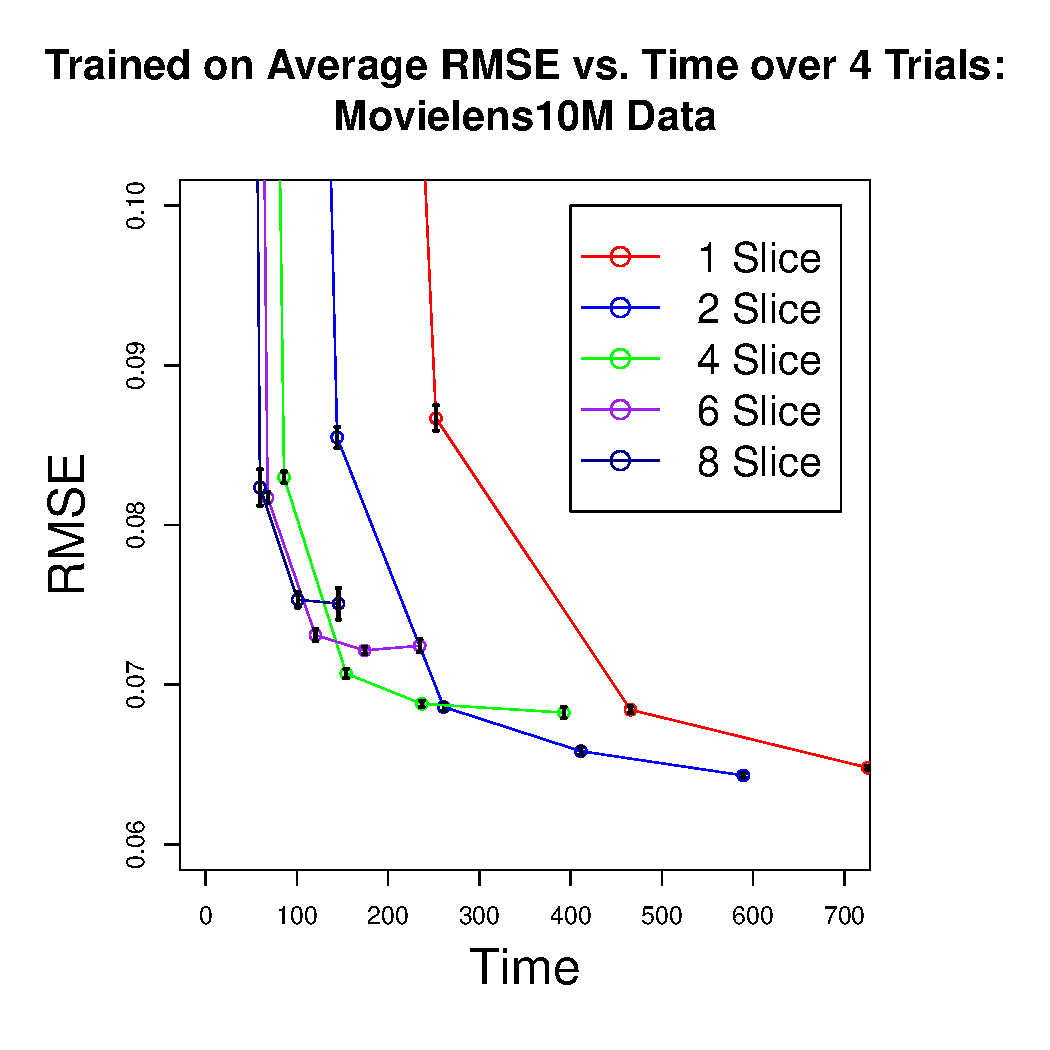
\includegraphics[width=\textwidth]{4000_90_1_to_4_RvT_graph.pdf}}
		\caption{Training Data.}
\end{center}
	\end{subfigure}
\hspace{1cm}
	\begin{subfigure}[b]{.45\textwidth}
\begin{center}
		\fbox{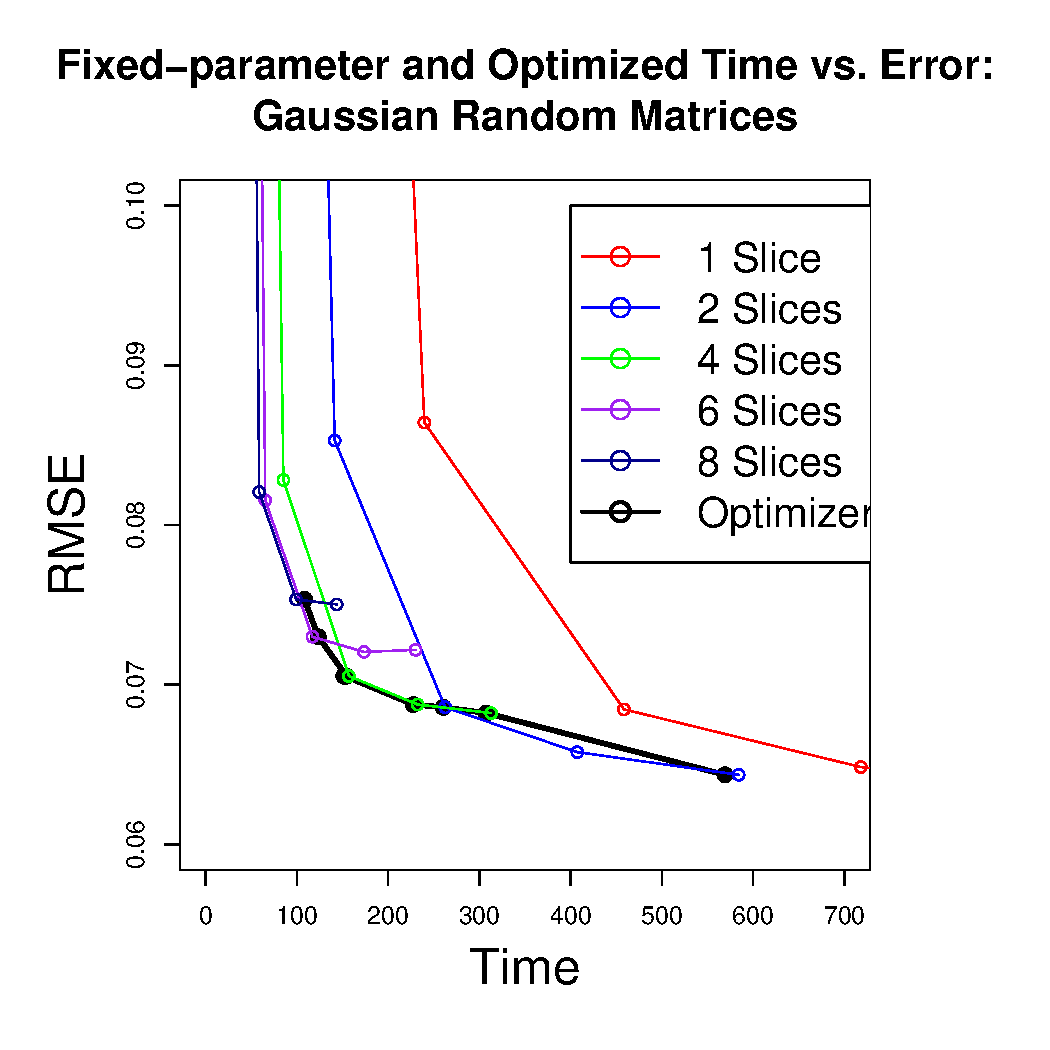
\includegraphics[width=\textwidth]{Opt_Gaussian_4000.pdf}}
		\caption{Testing Data.}
\end{center}
	\end{subfigure}
\hfill
	\caption{Plots of Time and Error taken to factor a 4000 by 4000 matrix drawn from a Gaussian distribution.}	
\end{figure}

\item MovieLens 10M Dataset (7 partitions, trained on 6, tested on 1)
\begin{figure}
	\begin{subfigure}[b]{.45\textwidth}
\begin{center}
		\fbox{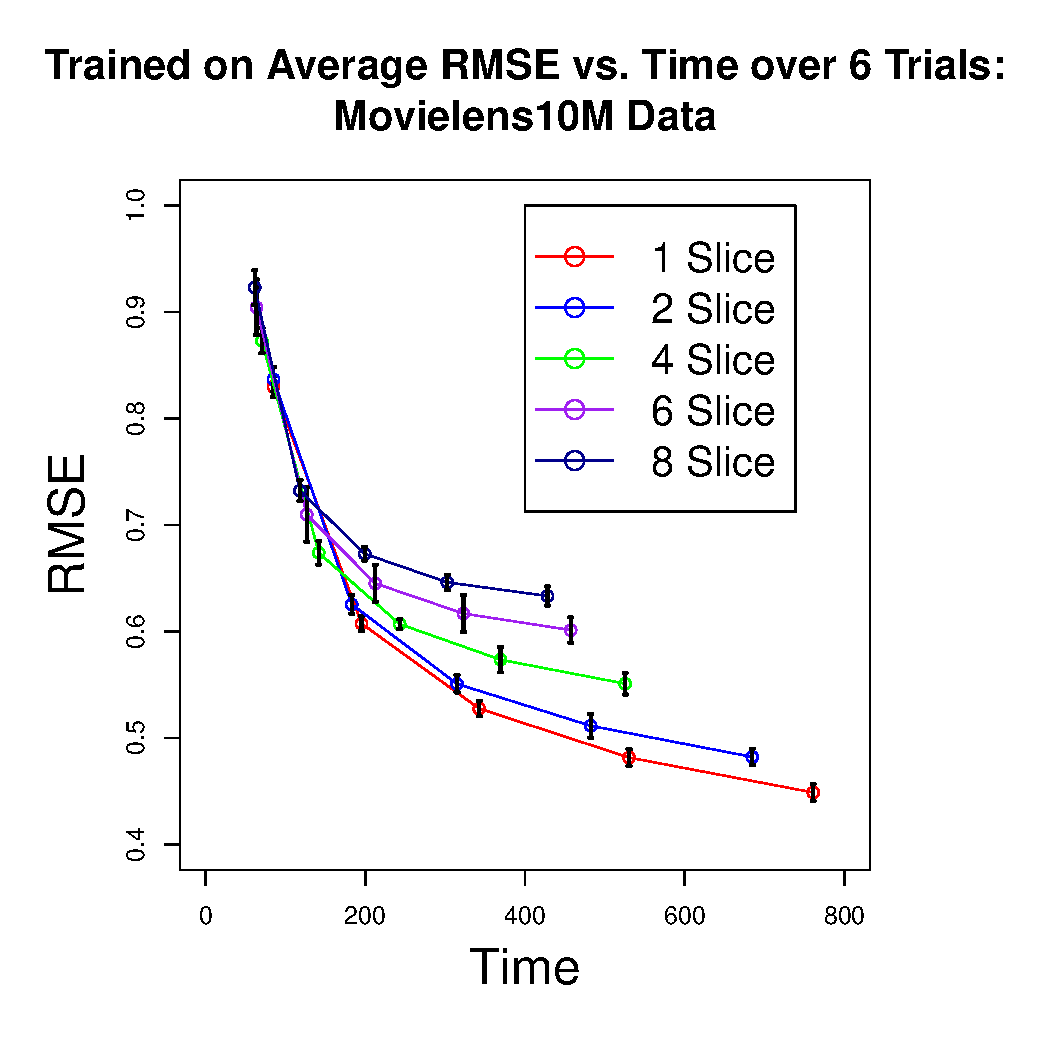
\includegraphics[width=\textwidth]{movielens10M_1_to_4_RvT_graph.pdf}}
		\caption{Training Data.}
\end{center}
	\end{subfigure}
\hspace{1cm}
	\begin{subfigure}[b]{.45\textwidth}
\begin{center}
		\fbox{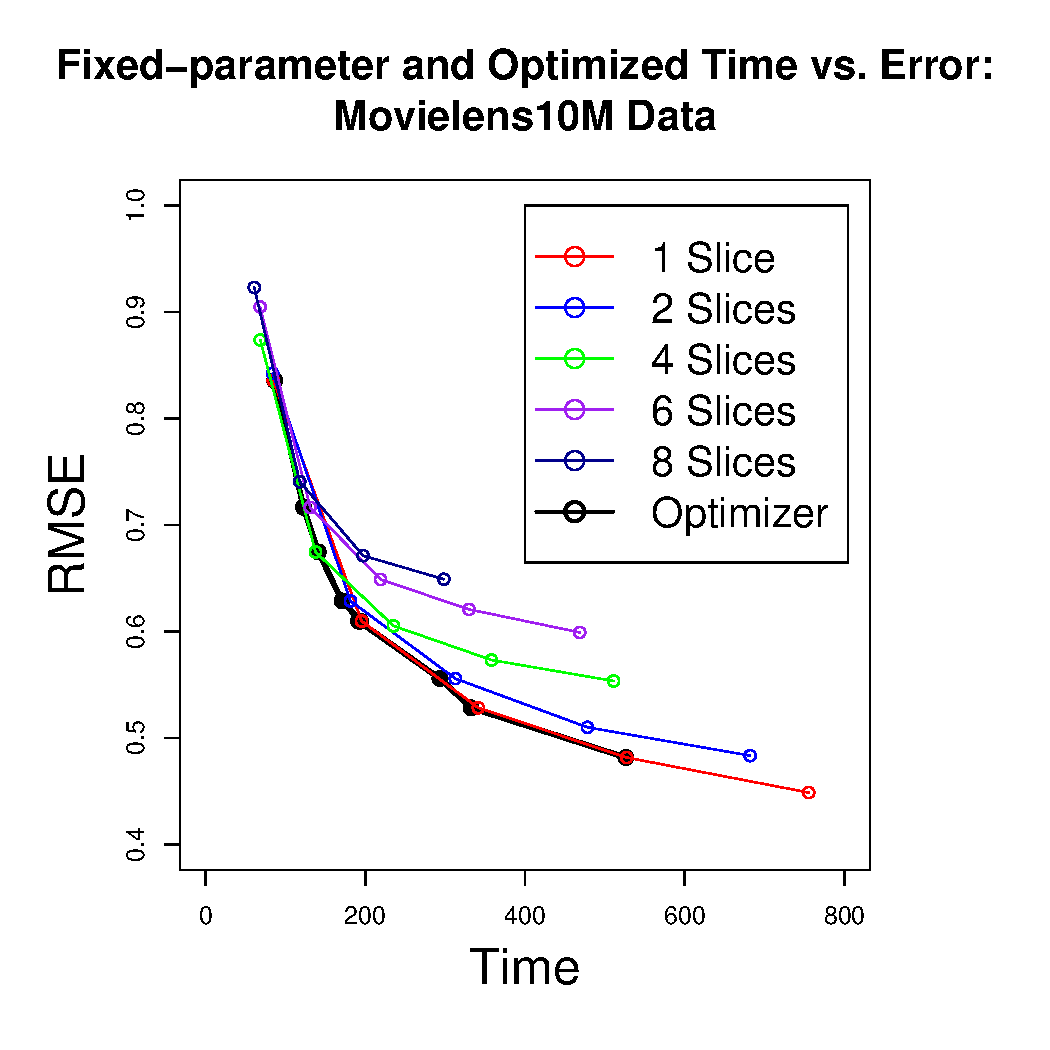
\includegraphics[width=\textwidth]{Opt_movielens.pdf}}
		\caption{Testing Data. }
\end{center}
	\end{subfigure}
\hfill
	\caption{Plots of Time and Error taken to factor a the Movielens 10M Datasetpartitions.}	
\end{figure}
\item Optimizer performs as well as manually setting the parameter!}
\end{itemize}

\vspace{1cm}

    \end{block}

\vspace{1.5cm}

    \begin{block}{\huge Future Work and Acknowledgements}
	\vspace{4mm}
{\Large Directions for further work include:}
\begin{itemize} {\Large
\item Optimize over space of algorithms
%\item Avoid RAM bottlenecks by distributing collect step
\item Handle novel jobs from new distributions (coming soon)}
\end{itemize}
	\vspace{4mm}
{\Large Our very warm thanks to:}
\begin{itemize} {\Large
\item Professors Anthony Joseph and John Kubiatowicz
\item Ameet Talwalkar and Shivaram Venkataraman for mentoring us
\item UC Berkeley and the NSF for providing funds and resources}
\vspace{.5cm}
\end{itemize}
    \end{block}
\end{column}

\end{columns}
\end{center}
\vspace{1.5cm}
  \end{frame}
  \end{document}
